\documentclass[Orbiter User Manual.tex]{subfiles}
\begin{document}

\section{User interface}
\label{sec:user_interface}
This section describes the keyboard, mouse and joystick interfaces for controlling spacecraft and other functions in Orbiter.


\subsection{Keyboard interface}
This section describes the \textit{default} Orbiter keyboard assignments. Please note that the assignments are customisable by editing the keymap.dat file in the Orbiter directory, and that therefore the keyboard controls for your Orbiter installation may be different.\\
The key assignments referenced in this section and the rest of the manual refer to the keyboard layout shown in the figure below. For other layouts (e.g. language-specific) the key labels may be different. The relevant criterion for key functions in Orbiter is the \textit{position of the key} on the keyboard, not the label. For example, on the German keyboard the keys for the "turn orbit-normal" (\keystroke{;}) and "turn orbit-antinormal" (\keystroke{'}) functions will be \keystroke{Ö} and \keystroke{Ä}.

\begin{figure}[H]
	\centering
	\subfigure{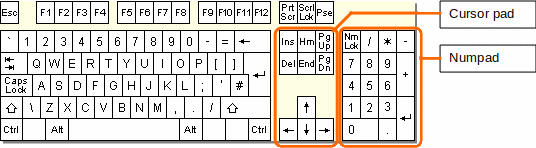
\includegraphics[width=0.75\textwidth]{keyboard.png}}
	\caption{Keyboard layout reference}
\end{figure}

\noindent
Note that certain spacecraft may define additional keyboard functions. Check individual documentation for a detailed description of spacecraft controls and functionality.\\
\\
\textbf{General}

%\begin{table}[H]
	%\centering
	\begin{longtable}{ |p{0.17\textwidth}|p{0.77\textwidth}| }
	\hline\rule{0pt}{2ex}
	\keystroke{R} & Time deceleration: Slow down the simulation speed by factor 10, to a minimum of 0.1x real time. See also \ref{ssec:menu_time}.\\
	\hline\rule{0pt}{2ex}
	\keystroke{T} & Time acceleration: Speed up the simulation time by a factor 10, to a maximum of 100000x real time. See also \ref{ssec:menu_time}.\\
	\hline\rule{0pt}{2ex}
	\keystroke{X} & Zoom camera out (increase field of view). See also \ref{ssec:menu_camera}.\\
	\hline\rule{0pt}{2ex}
	\keystroke{Z} & Zoom camera in (decrease field of view). See also \ref{ssec:menu_camera}.\\
	\hline\rule{0pt}{2ex}
	\Ctrl\keystroke{X} & Zoom out (in discrete steps of 10°).\\
	\hline\rule{0pt}{2ex}
	\Ctrl\keystroke{Z} & Zoom in (in discrete steps of 10°).\\
	\hline\rule{0pt}{2ex}
	\Ctrl\keystroke{C} & Start/stop recording a flight, or stop a playback. See also \ref{sec:flight_rec}.\\
	\hline\rule{0pt}{2ex}
	\Ctrl\keystroke{D} & Undock from a vessel.\\
	\hline\rule{0pt}{2ex}
	\Ctrl\keystroke{P} & Pause/resume simulation.\\
	\hline\rule{0pt}{2ex}
	\Ctrl\keystroke{Q} & Exit the simulation to the Launchpad window.\\
	\hline\rule{0pt}{2ex}
	\Ctrl\keystroke{S} & Quicksave the current simulation state to a scenario.\\
	\hline\rule{0pt}{2ex}
	\keystroke{F1} & Toggle cockpit/external view of the user-controlled spacecraft.\\
	\hline\rule{0pt}{2ex}
	\Ctrl\keystroke{F1} & Open the Camera dialog (see \ref{ssec:menu_camera}) to select camera target, view mode and field of view.\\
	\hline\rule{0pt}{2ex}
	\Alt\keystroke{F1} & Open the help window (see \ref{ssec:menu_help}).\\
	\hline\rule{0pt}{2ex}
	\keystroke{F2} & Cycle through external tracking view modes: target-relative / absolute direction / global frame (see \ref{ssec:menu_camera}).\\
	\hline\rule{0pt}{2ex}
	\Ctrl\keystroke{F2} & Open the Time acceleration dialog (see \ref{ssec:menu_time}).\\
	\hline\rule{0pt}{2ex}
	\keystroke{F3} & Open the vessel selection dialog (see \ref{ssec:menu_vessel_sel}).\\
	\hline\rule{0pt}{2ex}
	\Ctrl\keystroke{F3} & Switch control back to the previous vessel, if any. Allows jumping backwards and forwards between the last two vessels.\\
	\hline\rule{0pt}{2ex}
	\keystroke{F4} & Main menu (see \ref{sec:menu}).\\
	\hline\rule{0pt}{2ex}
	\Ctrl\keystroke{F4} & Open the Custom functions dialog for access to plug-in functions and dialogs (see \ref{ssec:menu_cust_func}).\\
	\hline\rule{0pt}{2ex}
	\Ctrl\keystroke{F5} & Open the Flight recorder/player dialog containing recording and playback functions (see \ref{sec:flight_rec}).\\
	\hline\rule{0pt}{2ex}
	\Ctrl\keystroke{I} & Open the Object info dialog (see \ref{ssec:menu_info}).\\
	\hline\rule{0pt}{2ex}
	\Ctrl\keystroke{M} & Open the Map window (see \ref{ssec:menu_map}).\\
	\hline\rule{0pt}{2ex}
	\keystroke{F9} & Toggle planetarium mode on/off (see \ref{ssec:menu_options}).\\
	\hline\rule{0pt}{2ex}
	\Ctrl\keystroke{F9} & Open the Visual helpers dialog for planetarium, force and axis display options (see \ref{ssec:menu_options}).\\
	\hline
	\end{longtable}
%\end{table}

\noindent
\\
\textbf{Spacecraft controls}\\
These keys allow manual manoeuvring of the user-controlled spacecraft. See also joystick controls. Note that some spacecraft may not define all thruster types.\\
\\
\underline{Main/retro thruster controls:}

%\begin{table}[H]
	%\centering
	\begin{longtable}{ |p{0.17\textwidth}|p{0.77\textwidth}| }
	\hline\rule{0pt}{2ex}
	\Ctrl\keystroke{+}$_{Num}$ & Accelerate by increasing main thruster setting or by decreasing retro thruster setting.\\
	\hline\rule{0pt}{2ex}
	\Ctrl\keystroke{-}$_{Num}$ & Decelerate by decreasing main thruster setting or by increasing retro thruster setting.\\
	\hline\rule{0pt}{2ex}
	\keystroke{*}$_{Num}$ & Cut off main and retro thrusters.\\
	\hline\rule{0pt}{2ex}
	\keystroke{+}$_{Num}$ & Fire main thrusters at 100\% while pressed (overrides permanent setting)\\
	\hline\rule{0pt}{2ex}
	\keystroke{-}$_{Num}$ & Fire retro thrusters at 100\% while pressed (overrides permanent setting)\\
	\hline
	\end{longtable}
%\end{table}

\noindent
\\
\underline{Hover thruster controls (where available):}

%\begin{table}[H]
	%\centering
	\begin{longtable}{ |p{0.17\textwidth}|p{0.77\textwidth}| }
	\hline\rule{0pt}{2ex}
	\keystroke{0}$_{Num}$ & Increase hover thruster setting.\\
	\hline\rule{0pt}{2ex}
	\keystroke{.}$_{Num}$ & Decrease hover thruster setting.\\
	\hline
	\end{longtable}
%\end{table}

\noindent
\\
\underline{Attitude thruster controls (rotational mode):}

%\begin{table}[H]
	%\centering
	\begin{longtable}{ |p{0.17\textwidth}|p{0.77\textwidth}| }
	\hline\rule{0pt}{2ex}
	\keystroke{4}/\keystroke{6}$_{Num}$ & Fire thrusters for rotation around longitudinal axis (bank).\\
	\hline\rule{0pt}{2ex}
	\keystroke{2}/\keystroke{8}$_{Num}$ & Fire thrusters for rotation around transversal axis (pitch).\\
	\hline\rule{0pt}{2ex}
	\keystroke{1}/\keystroke{3}$_{Num}$ & Fire thrusters for rotation around vertical axis (yaw).\\
	\hline\rule{0pt}{2ex}
	\keystroke{5}$_{Num}$ & Toggle \textit{kill} rotation autopilot mode: stops spacecraft rotation by engaging appropriate attitude thrusters.\\
	\hline
	\end{longtable}
%\end{table}

\noindent
\\
\underline{Attitude thruster controls (linear mode):}

%\begin{table}[H]
	%\centering
	\begin{longtable}{ |p{0.17\textwidth}|p{0.77\textwidth}| }
	\hline\rule{0pt}{2ex}
	\keystroke{2}/\keystroke{8}$_{Num}$ & Fire thrusters for up/down acceleration (along vertical axis).\\
	\hline\rule{0pt}{2ex}
	\keystroke{1}/\keystroke{3}$_{Num}$ & Fire thrusters for left/right acceleration (along transversal axis).\\
	\hline\rule{0pt}{2ex}
	\keystroke{6}/\keystroke{9}$_{Num}$ & Fire thrusters for forward/back acceleration (along longitudinal axis).\\
	\hline
	\end{longtable}
%\end{table}

\noindent
\\
Note: In combination with \Ctrl, thrusters are engaged at 10\% max. thrust for fine control.\\
\\
\underline{Other controls:}

%\begin{table}[H]
	%\centering
	\begin{longtable}{ |p{0.17\textwidth}|p{0.77\textwidth}| }
	\hline\rule{0pt}{2ex}
	\keystroke{/}$_{Num}$ & Toggle reaction control system between rotational and linear modes.\\
	\hline\rule{0pt}{2ex}
	\Ctrl\keystroke{/}$_{Num}$ & Enable/disable reaction control system\\
	\hline\rule{0pt}{2ex}
	\Alt\keystroke{/}$_{Num}$ & Enable/disable manual user control (via keyboard or joystick) of aerodynamic control surfaces (elevator, rudder, ailerons) if available\\
	\hline\rule{0pt}{2ex}
	\keystroke{A} & Toggle \textit{hold altitude} autopilot mode. Maintain current altitude above the surface by means of hover thrusters only. This will fail if hover thrusters cannot compensate for gravitational acceleration, in particular at high bank angles. Combining this mode with the \textit{H-level} mode is therefore useful.\\
	\hline\rule{0pt}{2ex}
	\keystroke{L} & Toggle \textit{H-level} autopilot mode. Keeps the spacecraft level with the local horizon by modulating attitude thrusters.\\
	\hline\rule{0pt}{2ex}
	\keystroke{[} & Toggle \textit{prograde} attitude mode. Turns the spacecraft into its orbital velocity vector with attitude thrusters.\\
	\hline\rule{0pt}{2ex}
	\keystroke{]} & Toggle \textit{retrograde} attitude mode. Turns the spacecraft into its negative orbital velocity vector with attitude thrusters.\\
	\hline\rule{0pt}{2ex}
	\keystroke{;} & Toggle orbit-normal attitude mode. Turns the spacecraft normal to its orbital plane (into direction R x V)\\
	\hline\rule{0pt}{2ex}
	\keystroke{'} & Toggle orbit-antinormal mode. Turns the spacecraft anti-normal to its orbital plane (into direction -R x V)\\
	\hline\rule{0pt}{2ex}
	\keystroke{Ins}/\keystroke{Del}$_{Cur}$ & Trim control (only for vessels with aerodynamic control surfaces)\\
	\hline\rule{0pt}{2ex}
	\keystroke{,}/\keystroke{.} & Apply left/right wheel brake (where available)\\
	\hline
	\end{longtable}
%\end{table}

\noindent
\\
\textbf{External camera views}\\
\\
\underline{Tracking camera:}

%\begin{table}[H]
	%\centering
	\begin{longtable}{ |p{0.17\textwidth}|p{0.77\textwidth}| }
	\hline\rule{0pt}{2ex}
	\keystroke{PageUp}$_{Cur}$ & Move camera away from target object.\\
	\hline\rule{0pt}{2ex}
	\keystroke{PageDown}$_{Cur}$ & Move camera towards target object.\\
	\hline\rule{0pt}{2ex}
	\Ctrl\UArrow\DArrow\RArrow\LArrow$_{Cur}$ & Rotate camera around target.\\
	\hline
	\end{longtable}
%\end{table}

\noindent
\\
\underline{Ground-based camera:}

%\begin{table}[H]
	%\centering
	\begin{longtable}{ |p{0.17\textwidth}|p{0.77\textwidth}| }
	\hline\rule{0pt}{2ex}
	\Ctrl\UArrow\DArrow\RArrow\LArrow$_{Cur}$ & Pan camera (free mode)\\
	\hline\rule{0pt}{2ex}
	\UArrow\DArrow\RArrow\LArrow$_{Cur}$ & Tilt camera (free mode)\\
	\hline\rule{0pt}{2ex}
	\RArrow\LArrow$_{Cur}$ & Rotate camera around target (target-locked mode)\\
	\hline\rule{0pt}{2ex}
	\UArrow\DArrow$_{Cur}$ & Move camera towards/away from target (target-locked mode)\\
	\hline\rule{0pt}{2ex}
	\keystroke{PageUp}/\keystroke{PageDown}$_{Cur}$ & Raise/lower camera\\
	\hline
	\end{longtable}
%\end{table}

\noindent
\\
\textbf{Internal (cockpit) view}

%\begin{table}[H]
	%\centering
	\begin{longtable}{ |p{0.17\textwidth}|p{0.77\textwidth}| }
	\hline\rule{0pt}{2ex}
	\keystroke{F8} & Cycle through generic (glass cockpit), 2D panel and 3D virtual cockpit views (if supported by the spacecraft)\\
	\hline\rule{0pt}{2ex}
	\Alt\UArrow\DArrow\RArrow\LArrow$_{Cur}$ & Rotate pilot view direction.\\
	\hline\rule{0pt}{2ex}
	\Home & Return to default (forward) pilot view direction.\\
	\hline\rule{0pt}{2ex}
	\Ctrl\Alt\UArrow\DArrow\RArrow\LArrow$_{Cur}$ & Lean left/right forward, return to default position (3D virtual cockpit only)\\
	\hline\rule{0pt}{2ex}
	\Ctrl\UArrow\DArrow\RArrow\LArrow$_{Cur}$ & Switch to next observer (pilot/crew/passengers) if available (3D virtual cockpit only)\\
	\hline\rule{0pt}{2ex}
	\UArrow\DArrow\RArrow\LArrow$_{Cur}$ & Scroll panel (2D panel view only)\\
	\hline\rule{0pt}{2ex}
	\Ctrl\UArrow\DArrow\RArrow\LArrow$_{Cur}$ & Switch to neighbour panel if present  (2D panel view only)\\
	\hline\rule{0pt}{2ex}
	\Ctrl\keystroke{H} & Toggle HUD display on/off.\\
	\hline\rule{0pt}{2ex}
	\Alt\keystroke{H} & Cycle through HUD colours.\\
	\hline\rule{0pt}{2ex}
	\keystroke{H} & Cycle through HUD modes.\\
	\hline\rule{0pt}{2ex}
	\Ctrl\keystroke{R} & HUD reference selection. (Orbit HUD: opens reference selection input box; Docking HUD: cycles through available NAV receivers)\\
	\hline\rule{0pt}{2ex}
	\Ctrl\Alt\keystroke{R} & Docking HUD only: Reference selection, bypassing XPDR and IDS transmitters\\
	\hline
	\end{longtable}
%\end{table}

\noindent
\\
\textbf{MFD control}\\
MFD functions are generally executed with \Shift-key combinations, where the left and right \Shift keys address the left and right standard MFD instruments, respectively.

%\begin{table}[H]
	%\centering
	\begin{longtable}{ |p{0.17\textwidth}|p{0.77\textwidth}| }
	\hline\rule{0pt}{2ex}
	\Shift\keystroke{Esc} & Toggle MFD on/off (presses the MFD PWR button)\\
	\hline\rule{0pt}{2ex}
	\Shift\keystroke{F1} & Cycle through all MFD mode selection pages, then jump back to current mode.\\
	\hline\rule{0pt}{2ex}
	\Shift\keystroke{'} & Toggle MFD menu page, listing descriptions for all function buttons.\\
	\hline\rule{0pt}{2ex}
	\Shift<mode> & On MFD mode selection pages only: \Shift in combination with a valid mode key selects that mode (see \ref{sec:mfd}).\\
	\hline\rule{0pt}{2ex}
	\Shift<func> & In standard display mode \Shift in combination with a valid mode-specific function key executes that function (see \ref{sec:mfd}).\\
	\hline
	\end{longtable}
%\end{table}

\noindent
\\
\textbf{Menu selections}

%\begin{table}[H]
	%\centering
	\begin{longtable}{ |p{0.17\textwidth}|p{0.77\textwidth}| }
	\hline\rule{0pt}{2ex}
	\UArrow$_{Cur}$ & Move to previous item in the list.\\
	\hline\rule{0pt}{2ex}
	\DArrow$_{Cur}$ & Move to next item in the list.\\
	\hline\rule{0pt}{2ex}
	\RArrow$_{Cur}$ & Display sub-list for the selected item if available.\\
	\hline\rule{0pt}{2ex}
	\LArrow$_{Cur}$ & Go back to the parent list from a sub-list.\\
	\hline\rule{0pt}{2ex}
	\Enter & Select the current item and close the list.\\
	\hline\rule{0pt}{2ex}
	\keystroke{Esc} & Close list.\\
	\hline
	\end{longtable}
%\end{table}


\subsection{Joystick interface}
A joystick can be used to operate the attitude and main thrusters, or the equivalent aerodynamic control surfaces (if available) of the user-controlled spacecraft manually.

%\begin{table}[H]
	%\centering
	\begin{longtable}{ |p{0.3\textwidth}|p{0.64\textwidth}| }
	\hline\rule{0pt}{2ex}
	\textbf{Action} & \textbf{Effect}\\
	\hline\rule{0pt}{2ex}
	Push stick left or right & Engage ailerons or engage RCS for rotation around longitudinal axis (bank)\\
	\hline\rule{0pt}{2ex}
	Push stick forward or back & Engage elevators or engage RCS for rotation around transversal axis (pitch)\\
	\hline\rule{0pt}{2ex}
	Operate rudder control or push stick left or right while holding joystick button 2 & Engage rudder or engage RCS for rotation around vertical axis (yaw)\\
	\hline\rule{0pt}{2ex}
	Operate throttle control & Set main thrust. Similar to \Ctrl\keystroke{+}$_{Num}$ and \Ctrl\keystroke{-}$_{Num}$ keyboard controls, but does not engage retro thrusters.\\
	\hline\rule{0pt}{2ex}
	Direction controller ("coolie hat") & Cockpit view: rotate pilot view direction\newline
	External view: rotate camera around target\\
	\hline\rule{0pt}{2ex}
	Direction controller + joystick button 2 & Cockpit view: scroll instrument panel (2D panel view only)\newline
	External view: tilt view direction (free ground observer view only)\\
	\hline
	\end{longtable}
%\end{table}


\subsection{Mouse interface}
Spacecraft instrument panels can be operated with the mouse. Most buttons, switches and dials are activated by clicking the left mouse button. Some elements like multi-way dials may respond to both left and right mouse clicks. In generic (glass cockpit) view, the buttons around the MFD displays can be operated with the mouse.\\
In external camera modes, the mouse wheel can be used to move the camera towards or away from the target.\\
In cockpit views, the mouse wheel changes the field of view (a good way to zoom an instrument display closer in the virtual cockpit). In addition, in 2-D panel cockpit views, \Ctrl + mouse wheel zooms the panel in and out if the native resolution of the panel is higher than the size of the simulation window (not supported for legacy panel implementations).\\
The camera direction can be rotated by pressing the right mouse button and dragging the mouse. This works both in external and cockpit views.

%\begin{table}[H]
	%\centering
	\begin{longtable}{ |p{0.3\textwidth}|p{0.64\textwidth}| }
	\hline\rule{0pt}{2ex}
	\textbf{Action} & \textbf{Effect}\\
	\hline\rule{0pt}{2ex}
	Left mouse button & Operate instruments in cockpit views\\
	\hline\rule{0pt}{2ex}
	Right mouse button + drag & Rotate camera view\\
	\hline\rule{0pt}{2ex}
	Mouse wheel & Cockpit view: Change camera field of view (FoV). See \keystroke{X}/\keystroke{Z}.\newline
	External track views: move camera toward/away from target.\\
	\hline\rule{0pt}{2ex}
	\Ctrl + mouse wheel & 2D panel view only: Zoom instrument panel in/out\\
	\hline
	\end{longtable}
%\end{table}


\subsection{Physical measures, units and magnitudes}
Orbiter and the associated documentation (including this manual) use \textit{SI units} (Système international), sometimes called the \textit{metric system}, for all default displays and calculations, with very few exceptions, e.g. \textit{days}, in particular in combination with MJD dates, or \textit{AU} (astronomical units) for distances on interplanetary scales. Another exception are angles, which are mostly displayed in degrees [°] instead of radians [rad].\\
Some of the frequently encountered base and derived units are

%\begin{table}[H]
	%\centering
	\begin{longtable}{ |p{0.22\textwidth}|p{0.72\textwidth}| }
	\hline\rule{0pt}{2ex}
	Time & second [s]\\
	\hline\rule{0pt}{2ex}
	Length & meter [m]\\
	\hline\rule{0pt}{2ex}
	Mass & kilogram [kg]\\
	\hline\rule{0pt}{2ex}
	Temperature & Kelvin [K]\\
	\hline\rule{0pt}{2ex}
	Speed & [m s$^{-1}$]\\
	\hline\rule{0pt}{2ex}
	Acceleration & [m s$^{-2}$]\\
	\hline\rule{0pt}{2ex}
	Linear momentum & [kg m s$^{-1}$]\\
	\hline\rule{0pt}{2ex}
	Angular momentum & [kg m$^{2}$ s$^{-1}$]\\
	\hline\rule{0pt}{2ex}
	Force & Newton [N]: 1 N = 1 kg m s$^{-2}$\\
	\hline\rule{0pt}{2ex}
	Energy, heat & Joule [J]: 1 J = 1 kg m$^{2}$ s$^{-2}$\\
	\hline\rule{0pt}{2ex}
	Power & Watt [W]: 1 W = 1 kg m$^{2}$ s$^{-3}$\\
	\hline\rule{0pt}{2ex}
	Pressure & Pascal [Pa]: 1 Pa = 1 N m$^{-2}$\\
	\hline\rule{0pt}{2ex}
	Frequency & Hertz [Hz]: 1 Hz = 1 s$^{-1}$\\
	\hline
	\end{longtable}
%\end{table}

\noindent
In MFD displays (see \ref{sec:mfd}) the units are generally omitted in numerical readouts of physical properties unless non-standard units are used.\\
Note that the instruments of specific spacecraft (in particular representations of historic vessels) may be calibrated in different unit systems. Always read the documentation of your vessel if in doubt.\\
\\
\textbf{Magnitudes}\\
Orbiter uses either the standard scientific notation (a $\cdot$ 10$^{b}$) or a magnitude suffix character (in particular in MFD displays when space is limited) to represent a range of magnitudes of the represented properties.

%\begin{table}[H]
	%\centering
	\begin{longtable}{ |p{0.22\textwidth}|p{0.72\textwidth}| }
	\hline\rule{0pt}{2ex}
	10$^{-9}$ & n (nano)\\
	\hline\rule{0pt}{2ex}
	10$^{-6}$ & u (micro)\\
	\hline\rule{0pt}{2ex}
	10$^{-3}$ & m (milli)\\
	\hline\rule{0pt}{2ex}
	10$^{3}$ & k (kilo)\\
	\hline\rule{0pt}{2ex}
	10$^{6}$ & M (mega)\\
	\hline\rule{0pt}{2ex}
	10$^{9}$ & G (giga)\\
	\hline
	\end{longtable}
%\end{table}

\noindent
Examples:

\begin{itemize}
\item A time period of 1.4k represents 1.4 $\cdot$ 10$^{3}$ s or 23 minutes 20 seconds.
\item A distance of 2.83G represents 2.83 $\cdot$ 10$^{9}$ m or 2830000 km
\item A mass of 4.7k represents 4.7 $\cdot$ 10$^{3}$ kg or 4.7 tons (note that the "k" in kg is part of the unit, not a magnitude suffix).
\item A pressure of 2.24m represents 2.24 $\cdot$ 10$^{-3}$ Pa.
\end{itemize}

\noindent
\\
\textbf{Precision and error limits}\\
Most displays don't provide explicit error estimates of the shown values. However, the precision of the numerical representation should be indicative of the confidence margins. Therefore, a value displayed as 1.32 should imply an error range of the order 1.32 $\pm$ 0.01, and 4.2k should be understood as (4.2 $\pm$ 0.1)k.



\end{document}
